\documentclass[twoside,11pt]{article}

% Any additional packages needed should be included after jmlr2e.
% Note that jmlr2e.sty includes epsfig, amssymb, natbib and graphicx,
% and defines many common macros, such as 'proof' and 'example'.
%
% It also sets the bibliographystyle to plainnat; for more information on
% natbib citation styles, see the natbib documentation, a copy of which
% is archived at http://www.jmlr.org/format/natbib.pdf

\usepackage{jmlr2e}
\usepackage{braket}
\usepackage[]{algorithm2e}
\usepackage{multirow}
\usepackage{mathrsfs}
\usepackage[Symbol]{upgreek}
\usepackage{mathtools}
\usepackage{fancyref}
\usepackage{graphicx}
%\usepackage{placeins}
\usepackage{subcaption}
\usepackage{fixltx2e}
% Definitions of handy macros can go here

\newcommand{\dataset}{{\cal D}}
\newcommand{\fracpartial}[2]{\frac{\partial #1}{\partial  #2}}

% Heading arguments are {volume}{year}{pages}{submitted}{published}{author-full-names}

\jmlrheading{1}{2000}{1-48}{4/00}{10/00}{Name and Name}

% Short headings should be running head and authors last names

\ShortHeadings{Imitation Learning for Accelerating Fixed Point Iterative Processes }{Name and Name}
\firstpageno{1}

\begin{document}

\title{Imitation Learning for Accelerating Fixed Point Iterative Processes}
%title{Speeding up Hartree-Fock by Imitation Learning}

\author{\name Name\ Name \email email \\
       \addr Department\\
       University \\
       City, State , USA
       \AND
       \name Name\ Name \email email \\
       \addr Department\\
       University \\
       City, State , USA}
\editor{editor name}

\maketitle


\begin{abstract}
A means to accelerate iterative processes by using imitation learning is provided. This work focuses on the application of quantum mechanics and solving Hartree-Fock, which is a method for approximating the electron distribution and energy of a given molecular system. Hartree-Fock is excessively time-consuming or even infeasible when applied to large molecules. Besides, depending on input, it is not always guaranteed to converge to a solution. Speeding up Hartree-Fock and making it more robust would thus enable scientists to deal with more complicated molecules and study chemical reactions with larger systems. In the present work, we attempt to improve on Hartree-Fock by imitation learning: from the trajectory produced by the original Hartree-Fock, we extract an (expensive to evaluate) expert policy which converges to a solution quickly and reliably, and attempt to imitate this policy with a less-expensive policy class.  To solve the imitation learning problem, we apply the Dataset Aggregation algorithm (DAgger), which learns a policy that is guaranteed to perform well under its induced distribution of states. In the experiment, we show that after 
%applying one iteration of DAgger, we got a faster convergence. 
 multiple iterations of DAgger, the performance improves and becomes less over-fit. 
\end{abstract}

\section{INTRODUCTION}

% Geoff: Is phrasing "enhanced expert demonstration" good?
Many computational methods in science and engineering use fixed-point iteration
\[
x_{n+1} = f(x_n), \quad n = 0,1,2,3...
\]
to attempt to find fixed points of $f$, i.e. points at which $f(x)=x$. The iterations generate a sequence, $x_0, x_1, x_2, \ldots$, that ideally converge to a fixed point, $x$. This paper explores the application of imitation learning to fixed-point iteration to accelerate convergence and improve stability. Imitation learning, also called learning from demonstration, is designed to learn a policy that imitates an expert's demonstration so as to become capable of performing the task demonstrated by the expert. For many important problems in science and engineering, considerable effort have gone into developing and fine-tuning fixed-point iteration algorithms. The sequences generated from these existing algorithms, $x_0, x_1, x_2$  provide a basis for creating expert demonstrations with enhanced performance. For example, the series $x_0, x_2, x_4$ provides an enhanced expert demonstration with accelerated convergence. The use of imitation learning to discover policies that mimic the behavior of such enhanced experts has the potential to substantially improve algorithms that are at the core of much of computational science.

In the field of computational quantum chemistry, the Hartree-Fock method is a fixed-point algorithm that is used to approximate the electronic structure and energy of molecules. Hartree-Fock is a specific instance of a broader class of mean-field theory approaches to many-body problems. In such mean-field theories, the effect of all individuals on any given individual is approximated by a single averaged effect, thus reducing a many-body problem to a one-body problem. In quantum chemistry, the mean field arises from the averaged charge distribution of the electrons, as described by the electron density, $\rho({\bf r})$. The Hartree-Fock iterations thereby generate a series of electron densities that ideally converge to a fixed point. Quantum chemical methods that go beyond mean-field theory typically begin with the results of a Hartree-Fock calculation, making the Hartree-Fock algorithm a pervasive component of quantum chemistry.\cite{Some authoritative review of electronic-structure theory}

Here, well-established Hartree-Fock algorithms are used to generate series of electron densities from which enhanced expert demonstrations are constructed. We then apply supervised learning to train a policy that mimics the demonstration. However, naive supervised learning may yield poor performance in practice and also in theory.  Because the learner's prediction and action affect future observations and states during the execution of the learned policy, it obviously violates the common i.i.d. assumption made in most statistical learning approaches \citep{Ross}. Fortunately, the dataset aggregation algorithm (DAgger), proposed by Ross et al. \citep{DAgger}, can learn a stationary deterministic policy guaranteed to perform well under its induced distribution of states. This in turn serves as a remedy to the poor performance in naive supervised learning. DAgger also has been shown to have stable performance and fast learning rate \citep{DAggerCompare}. Below, DAgger is shown to yield policies whose performance is superior to those obtained from more naive approaches. 

\section{BACKGROUND}

\subsection{Hartree-Fock}

The core problem of quantum chemistry is to compute the electronic distribution, given the position of the nuclei. In Hartree-Fock theory, the distribution is described by the electron density, $\rho({\bf r})$, which gives the probability of finding any electron at the position ${\bf r}$. Hartree-Fock theory derives from the time-independent Schr\"{o}dinger equation,
\begin{equation} \label{eq:schrodinger}
				\hat{H}\Psi = E\Psi
\end{equation}
where $\hat{H}$ is the Hamiltonian operator and the many-body, or many-electron, wave-function $\Psi$ is an eigenfunction of that operator. Different $\Psi$'s correspond to different quantum states of the system, but the goal of Hartree-Fock theory is to approximate the lowest-energy state. [expand?]  Hartree-Fock theory uses a mean-field approach to convert the many-body Schr\"{o}dinger equation to a one-electron problem,
\begin{equation} \label{eq:fockSchrodinger}
				\hat{F}\phi_a({\bf r}) = \epsilon_a \phi_a({\bf r})
\end{equation}
where $\hat{F}$ is the Fock operator, $\phi_a({\bf r})$ are the molecular orbitals, which describe the possible quantum states of individual electrons, and $\epsilon_a$ are the molecular orbital energies. An approximation for the many-electron system is then constructed by assuming the $N$ electrons of the molecule occupy the lowest-energy orbitals, consistent with the Pauli exclusion principle restriction of placing at most two electrons (one with spin up and one with spin down) into any given molecular orbital. The Fock operator
\begin{equation} \label{eq:fock}
\hat{F}(\rho) = \hat{h}_1 + \hat{G}(\rho({\bf r}))
\end{equation}
where $\hat{h}_1$ is the one-electron Hamiltonian containing the operators that account for the kinetic energy of the electrons and the interaction of the electrons with the nuclei. $\hat{G}$ is an operator that captures the interaction between a single electron and the mean field resulting from all electrons. This mean field is constructed from the electron density, $\rho({\bf r})$. 

For computational expediency, the molecular orbitals, $\chi_a$ of Eq.~\ref{eq:fockSchrodinger} are written as a linear combination of atomic orbitals,
\begin{equation}\label{eq:lcao}
\phi_a({\bf r}) = \sum_{i=1}^{N_{basis}} \chi_i({\bf r}) C_{i,a}
\end{equation}
The set of basis functions provides a finite-dimensional Hilbert space in which to obtain approximate solutions. In this space, the operators $\hat{F}$, $\hat{h}_1$ and $\hat{G}$, along with the density $\rho({\bf r})$ become symmetric matrices of dimension $N_{basis}$ and Eq.~\ref{eq:fockSchrodinger} becomes a generalised matrix eigenvalue problem,
\begin{equation}\label{eq:fockMatrix}
F(\rho)C = SC\epsilon
\end{equation}
where $F$ is the Fock matrix and $S$ is the overlap matrix of inner products of the basis functions. $\rho$ is the density matrix which expresses the electron density $\rho(({\bf r})$ in the basis set and is given by $C^TC$. Hartree-Fock scales nominally as $N_{basis}^4$ due to the evaluation of $\hat{G}$, although scalings closer to $N_{basis}^3$ are routinely achieved by taking advantage of sparsity in construction of $\hat{G}$\ref{?}.


\begin{algorithm}[htb]
 \KwData{ 3D coordinates of atomic nuclei}
 \KwResult{Density matrix which gives minimum energy}
	Choose basis set of desired size \\
	Initialize $i \leftarrow	 0$ \\	
	Pick a starting density matrix $\rho_0$ \\
	Pick $\delta$ to be a small value (termination criteria) \\
 \While{ $i=0$ or $|E_{i} - E_{i-1}| > \delta$ }{
    Construct guess density matrix $\rho$ from available $\rho_i$ \\
	Calculate the Fock operator  $F \leftarrow h_1 + G(\rho)$\\
	Solve for $\epsilon$ and $C$ using Eq.~\ref{eq:fockMatrix} \\
	Update density matrix $\rho_{i+1}$ = $C^TC$\\
	$i \leftarrow i+1$ \\
 }
 \caption{Hartree-Fock algorithm}
\label{alg:hf}
\end{algorithm}

The corresponding fixed point iteration is shown in Algorithm\ref{alg:hf}. Implementations differ with regards to the means used to construct the starting density matrix and, more importantly for the current study, with regards to the means used to construct a guess density matrix from past iterates, $\rho_i$. This is typically done by taking a linear combination of these past iterates. In the Direct Inversion in the Iterative Subspace (DIIS) method\citep{Pulay1980}, the linear coefficients are chosen by associating an error vector which each iterate and choosing coefficients that minimize the summed error. Various methods have been used to define the error vector and to find the linear combinations that minimize the predicted error.~\citep{ADIIS,compScuseria,Alejandro2012} However, how to generate linear combinations that lead to the fastest convergence remains an open question\citep{Konstantin2002, Thorsten2011}. The current work retains the approach of using a linear combination of past iterates, but uses supervised learning to discover the optimal coefficients. 

%\subsection{Accelerating Hartree-Fock convergence as an imitation learning problem}

%The $n$ iterations of the Hartree-Fock process may be viewed as a sequence, beginning with the initial density matrix $\rho_0$, moving through $n-1$ intermediate density matrices $\rho_1$,  $\rho_2$,  $\ldots$ ,$\rho_{n-1}$ and finally ending at the steady-state converged output $\rho_{n}$. The only object that is needed is the final steady-state density matrix. If we can get this final density matrices with fewer iterations, the computation time would be shortened. An expert demonstration with twice the original convergence rate can be constructed, for example, by taking a step size of 2 over the original trajectory: $\rho_0 \rightarrow \rho_2 \rightarrow  \rho_4 \rightarrow  \ldots \rightarrow  \rho_{n}$. We can also construction greedier trajectories by taking larger step sizes or by moving directly to the steady-state density matrix from any starting point ($\rho_0 \rightarrow \rho_{n}$). 

%The connection to imitation learning is through the attempt to learn policies that map from any input density matrix to the next density matrix of one of these accelerated sequences. Below, these policies are invoked in the first line of the while loop in Algorithm~\ref{alg:hf}, where the density matrix to be used to compute the Fock matrix is constructed from the density matrices obtained from past iterations. 

\subsection{DAgger algorithm}
DAgger is an algorithm that learns from an expert demonstration in an iterative manner. In each iteration, a model is trained under the states that were induced by both the expert and the previous learned models. This aggregation expands the training to include inputs that the model is likely to encounter based on previous training iterations. By doing so, it is possible to offset the error made by previous learned models and thus learn a new policy that better approaches the demonstration. This is a remedy to the problem, in naive supervised learning, that the error may grow quadratically and results may become unpredictable because the policy is trained under a different state distribution than the model may encounter. 

The DAgger algorithm is given as Algorithm \ref{alg:DAgger}. $\Pi$ is the class of policies the learner is considering. In the first iteration, it uses the expert's policy $\pi^*$ to gather a dataset of trajectories $D$ and train a policy $\hat{\pi}_2$ that best mimics the expert on those trajectories. 

Then in iteration $i$, we sample states according to a mixture of policies ($\hat{\pi}_i$ and the expert $\pi^*$) and refer to expert's action on these states, forming the dataset $D_i$, which is in turn added to the overall dataset $D$. We then train the next policy $\hat{\pi}_{+1}$, the policy that best mimics the expert on the whole dataset $D$. The process is then repeated to further rectify the error produced by the policy learned in the previous iteration until we reach iteration $N$.

\begin{algorithm}[htb]
 \KwData{Expert's demonstration generated by expert's policy $\pi^*$}
 \KwResult{Best $\hat{\pi}_j$ on validation }
 $\pi^*$  is the expert’s policy \\
 Initialized $D \leftarrow \emptyset$ \\
 Initialized $\hat{\pi}_1$ to any policy in $\Pi$ \\
 \For{j=1 to N }{
	Let $\pi_i$ = $\beta_{j}\pi^* + (1-\beta_{j})\hat{\pi_j}$ \\
	Sample T-step trajectories using $\pi_j$ \\
	Get dataset $D_j$ = \{(s, $\pi^*$(s))\} of visited states by $\pi_j$ and actions given by expert. \\
	Aggregate datasets: $D \leftarrow D \cup D_j$ \\
	Train policy $\hat{\pi}_{j+1}$ on $D$\\
 }
 \caption{DAgger algorithm}
 \label{alg:DAgger}
\end{algorithm}

\section{LEARNING THE POLICY} \label{sec:policy}

\begin{center} 
	\begin{table*}[t]
	\footnotesize\setlength{\tabcolsep}{2.5pt}
	\renewcommand{\arraystretch}{1.5}
		\caption{Applying DAgger on the Expert's demonstration with step size = 2}
		\resizebox{\columnwidth}{!}{\begin{tabular}{|l|l|l|l|l|l|l|l|}
			\hline	\multicolumn{2}{|l|}{} & \multicolumn{6}{l|}{	Hartree-Fock iterations (with step size = 2)} \\ \hline	\multirow{10}{*}{
				\begin{tabular}[c]{@{}l@{}}DAgger\\ iterations\end{tabular}}	 
	&      iter          &                &  iter 1         & iter 2          & iter 3         & \ldots         & iter x = $\frac{n}{2}$         
	\\ \cline{2-8} 	& \multirow{2}{*}{ 1} 
	& Objective & $(\rho_0) \rightarrow \rho_2$ & $(\rho_0,\rho_2) \rightarrow \rho_4$ & $(\rho_0,\rho_2,\rho_4) \rightarrow \rho_6$ &  \ldots & $(\rho_{2i})_{i=0}^{x-1} \rightarrow \rho_{n}$ \\ \cline{3-8} 
	&                 & Result & ($\rho_0) \rightarrow \rho_2'$ & $(\rho_0,\rho_2)  \rightarrow \rho_4'$   & $(\rho_0,\rho_2,\rho_4) \rightarrow \rho_6'$    &  \ldots & $(\rho_{2i})_{i=0}^{x-1} \rightarrow \rho_{n}'$          \\ \cline{2-8} 
	& \multirow{2}{*}{ 2} & New objective         &                         & $(\rho_0,\rho_2')  \rightarrow \rho_4$   & $(\rho_0,\rho_2,\rho_4') \rightarrow \rho_6$     &  \ldots & $((\rho_{2i})_{i=0}^{x-2} ,\rho_{2(x-1)}')\rightarrow \rho_{n}$          \\ \cline{3-8} 
	&                 & Result &                 & $(\rho_0,\rho_2') \rightarrow \rho_4''$ & $(\rho_0,\rho_2,\rho_4') \rightarrow \rho_6''$   & \ldots & $((\rho_{2i})_{i=0}^{x-2} ,\rho_{2(x-1)}') \rightarrow \rho_{n}''$        \\ \cline{2-8} 
	& \multirow{2}{*}{ 3} & New objective         &                         &                          & $(\rho_0,\rho_2',\rho_4'')  \rightarrow \rho_6$    &  \ldots & $((\rho_{2i})_{i=0}^{x-3} ,(\rho_{2i}^{[i-(x-3)]})_{i=x-2}^{x-1}) \rightarrow \rho_{n}$         \\ \cline{3-8} 
	&                 & Result &                 &                 & $(\rho_0,\rho_2',\rho_4'')  \rightarrow \rho_6'''$ &  \ldots & $((\rho_{2i})_{i=0}^{n-3} ,(\rho_{2i}^{[i-(x-3)]})_{i=x-2}^{x-1})\rightarrow \rho_{n}'''$      \\ \cline{2-8} 
	& \vdots      & \vdots      &                &                &                & $\ddots$ &   \vdots \\ \cline{2-8} 
	& \multirow{2}{*}{ x=$\frac{n}{2}$} & New objective         &                         &                          &                            &  & $(\rho_{2i}^{[i]})_{i=0}^{x-1} \rightarrow \rho_{n}$     \\ \cline{3-8} 
	&                & Result  &                &                &                &  & $(\rho_{2i}^{[i]})_{i=0}^{x-1}\rightarrow \rho_{n}^{[x]}$ \\ \hline
	\end{tabular}}
	\label{tab:DAgger}
	\end{table*}
\end{center} 

The $n$ iterations of the Hartree-Fock process may be viewed as a sequence, beginning with the initial density matrix $\rho_0$, moving through $n-1$ intermediate density matrices $\rho_1$,  $\rho_2$,  $\ldots$ ,$\rho_{n-1}$ and finally ending at the steady-state converged output $\rho_{n}$. The only object that is needed is the final steady-state density matrix. If we can get this final density matrices with fewer iterations, the computation time would be shortened. An expert demonstration with an enhanced convergence rate can be constructed by, for example, taking a step size of 2 over the original trajectory: $\rho_0 \rightarrow \rho_2 \rightarrow  \rho_4 \rightarrow  \ldots \rightarrow  \rho_{n}$. We can also construct greedier trajectories by taking larger step sizes or by moving directly to the steady-state density matrix from any starting point ($\rho_0 \rightarrow \rho_{n}$). 

Accelerating Hartree-Fock can be cast as an imitation learning problem by attempting to learn policies that mimic experts with accelerated convergence, such as that with a step size of two over the original sequence of density matrices. These policies are invoked in the first line of the while loop in Algorithm~\ref{alg:hf}, where the density matrix to be used to compute the Fock matrix is constructed from the density matrices obtained from past iterations. Below, we consider policies where the new density matrix is written as a linear combination of past density matrices. The set of linear coefficients used to generate the guess density for the $i^{th}$ iteration of Hartree-Fock will be referred to as $\hat{c}_i$.

% What is the correct notation for the entire set of all $\hat{c}_i$
Referring to the DAgger algorithm, in our case, $\Pi$ is the policy class consisting of all modified Hartree-Fock methods, Algorithm~\ref{alg:hf}, in which a set of linear coefficients $\hat{c}_i$ is used to construct the input guess density matrix from past density matrices. $\pi^*$ represents the expert's policy that generates a sequence of density matrices with enhanced convergence. For the remainder of this paper, we consider the sequence $\rho_0 \rightarrow \rho_2 \rightarrow  \rho_4 \rightarrow  \ldots \rightarrow  \rho_{n}$. 


The main idea of DAgger is to train the policy under the induced state of the previous policies. Therefore, refer to the Algorithm~\ref{alg:DAgger}, when training policy $\hat{\pi}_{j+1}$ in DAgger iteration $j$, we will consider states generated from the previous policy $\hat{\pi}_{j}$ and all earlier policies. For convenience, we introduce the notation $(\rho_a, \rho_b, ....) \rightarrow \rho_c $ to represent the outcome of a single Hartree-Fock iteration, in which a linear combination of the density matrices $\rho_a, \rho_b, ....$ is used by Hartree-Fock to generate the next density matrix $\rho_c$ of the series. 

The training process is visualized in Table~\ref{tab:DAgger}, in which Hartree-Fock iterations are shown as columns and Dagger iterations are shown as rows. We begin by training a policy for the first iteration of Hartree-Fock. In this case DAgger has only one iteration, in which a policy is trained on the objective $(\rho_0) \rightarrow \rho_2$. The policy resulting from this training is specified by the linear coefficients $\hat{c}^{[1]}_1$, where the superscript indicates DAgger iteration and the subscript indicates Hartree-Fock iteration. The density matrices generated from this policy are referred to as $\rho_2^{'}$, where the number of primes indicates the DAgger iteration. 

The training process then moves onto the second Hartree-Fock iteration. In the first DAgger iteration, a policy is trained on $(\rho_0, \rho_2) \rightarrow \rho_4$. The resulting policy is specified by the linear coefficients $\hat{c}^{[1]}_2$ and generates induced states, $\rho_4^{'}$. In the second DAgger iteration, we include states induced from the training on the past Hartree-Fock iterations, by expanding the objective to include $(\rho_0, \rho_2^{'}) \rightarrow \rho_4$. The resulting policy is specified by the linear coefficients $\hat{c}^{[2]}_2$ and generates induced states, $\rho_4^{''}$. As this point, this are no additional induced states to include in the training and so the DAgger iteration terminates. 

This process continues on to the third Hartree-Fock iteration, which involves three DAgger iterations. The first iteration trains on only expert states $(\rho_0, \rho_2, \rho_4) \rightarrow \rho_6$, generating coefficients $\hat{c}^{[1]}_3$ and $\rho_6^{'}$. The second DAgger iteration expands the objective to include sequences in which the final input density matrix includes states induced by previous policies, $(\rho_0, \rho_2, \rho_4^{'}) \rightarrow \rho_6$. The third DAgger iteration adds sequences in which the states induced by the previous policies begin at the penultimate input density matrix,  $(\rho_0, \rho_2^{'}, \rho_{4}^{''}) \rightarrow \rho_6$. In general, each DAgger iteration expands the objective to includes sequences in which the induced states begin one step earlier than the previous DAgger iteration.  

This process of expanding the objective by aggregating previous sequences of induced states is the key to compensating the error made by the previous iterations. The training leads to policy that is expressed through the set of coefficients $\hat{c}^{[i]}_i$ that specify how to construct the guess density matrix for the $i^{th}$ Hartree-Fock iteration from the previous density matrices. This policy not only mimics the expert's demonstration but also offsets the error made by the previous iterations.

\section{EXPERIMENTAL DESIGN}

The computational experiments use the approach of Section~\ref{sec:policy} to train a policy for accelerating Hartree-Fock and compare the results to some baseline approaches. Of particular interest is the degree to which a policy trained on one class of molecules can transfer to a different class of molecules. 

\begin{figure}[h!]
\centering
\begin{subfigure}{.3\textwidth}
  \centering
  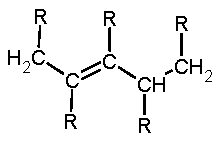
\includegraphics[width=80px]{pent3ene.pdf}
  \caption{Pent-3-ene}
  \label{fig:pent3ene}
\end{subfigure}%
\begin{subfigure}{.3\textwidth}
  \centering
  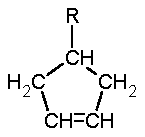
\includegraphics[width=60px]{RcycloPenteneHs.pdf}
  \caption{Cyclo-Pentene}
  \label{fig:cycloPen}
\end{subfigure}
\begin{subfigure}{.3\textwidth}
  \centering
  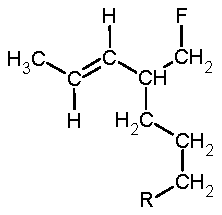
\includegraphics[width=80px]{pent3ene2propNOF.pdf}
  \caption{Pent-3-ene-2-propyl-1-F}
  \label{fig:propSub}
\end{subfigure}
\caption{The chemical structure of molecules in the datasets, R = H, F, OH or NH\textsubscript{2}}
\label{fig:Molecules}
\end{figure}

The following three data sets were generated, with the first being used for training and the remaining used for testing. Each data set consists of a set of molecules, as defined by the bonding pattern between the atoms, and a set of distinct molecular geometries of these molecules, as defined by distortions of the structure away from the equilibrium geometry at which the energy of the molecule is minimized. This geometric distortions are generated using a random uniform distribution of $\pm$0.5 \AA\ for bond lengths and $\pm$10\textsuperscript{o} for bond angles.  This approach of uniform sampling generates highly distorted structures. To prevent inclusion of structures that are of little interest in chemical applications, structures are rejected if there are contacts closer that 3\AA\ between non-bonded atoms.  In addition, each molecular configuration is placed in 4 different environments (1 with no environment + 3 different fields for X, Y and Z direction).
\begin{description}
\item[\textit{pent3ene}] 15 unique molecules corresponding to single substition of Pent-3-ene. Single substitution refers to placing a single substituent at one of the positions indicated by R in Figure~\ref{fig:pent3ene}, with all other R's being hydrogen (-H). The substituents are flourine (-F), hydroxyl (-OH) and amine (-NH\textsubscript{2}). The training set includes, for each molecule, the equilibrium geometry and three distorted geometries. The test set includes three distorted geometries for each molecule. Distortions include free rotation about leftmost carbon-carbon single bond of Figure~\ref{fig:pent3ene}. 
\item[\textit{cycloPentene}]Includes cyclo-pentene and its three singly-substituted analogues (Figure~\ref{fig:cycloPen}), each in the equilibrium geometry and 4 distorted geometries. 
\item[\textit{pentPropylF}] Includes the three singly-substituted species of pent-3-ene-2-propyl-1-Fluorine (Figure~\ref{fig:propSub}), each in its minimum-energy geometry and 7 distorted geometries. Distortions include free rotation about leftmost carbon-carbon single bond of Figure~\ref{fig:propSub}. 
\end{description}

%Geoff: Is R a form of regularization? 
For each molecular instance, the steady-state density matrix, $\rho_n$, is obtained using a standard fixed-point algorithm\cite{Pulay1980}. The learning objective is then defined as the sum of the distance of the density matrix, $\|\rho_i-\rho_n\|$, and the molecular energy, $|E(\rho_i)-E(\rho_n)|$ in Hartrees, from convergence. Because As in DIIS methods, it is likely desirable to have the coefficients of the linear combination of density matrices sum to one\cite{scusceria} the following is added to the objective,
\begin{equation}
R^{(i)}_j =  w [(\sum \|\hat{c}^{(i)}_j\| - 1]
\end{equation}
where the weight $w$ was empirically adjusted to a value of 30. 

%TODO: Is it single iteration DAgger? Ok to rename as no-induced-states
An expert demonstration that is optimal for the training data is then constructed as follows. We first train a policy that takes the initial density matrix to the final density matrix $(\rho_0) \rightarrow \rho_n$, and use this generate $\rho_1$. A policy is then trained on $(\rho_0, \rho_1) \rightarrow \rho_n$ and used to generate $\rho_2$. This approach is essentially single-iteration DAgger targetting $\rho_n$ and will be referred to as the ``no induced states'' policy. Every instance in the training data converges in less than 12 iterations, which is considerably faster than DIIS\cite{Pulay1980} and so provides a high-quality expert demonstration. Enhanced expert demonstrations are then created by eliminating the odd numbered iterations and DAgger is used to train a policy that mimics this enhanced demonstration, as in Section~\ref{sec:policy}. 

To further expand the training data, expert demonstrations are constructed starting from two different initial density matrices, $\rho_0$ of Algorithm~\ref{alg:hf} equal to 0 and to the identity matrix. This leads to two different expert demonstrations for each molecular instance that sample substantially different states in the initial trajectories. 
As a ``baseline'' policy for comparison, we use the simple, but still utilized, policy in which the density matrix for iteration $i$ is the average of the density matrices from the past two iterations.

\section{RESULTS}


\begin{figure}[h!]
\centering
\begin{subfigure}{.5\textwidth}
  \centering
  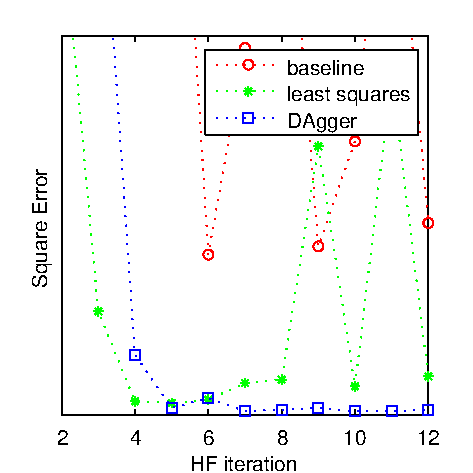
\includegraphics[scale=0.7]{cycloPen_pzero_test_12iter.pdf}
  \caption{$\rho_0 = 0$}
  \label{fig:cycloPen0}
\end{subfigure}%
\begin{subfigure}{.5\textwidth}
  \centering
  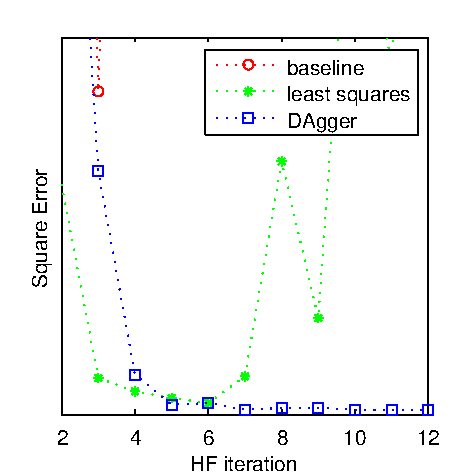
\includegraphics[scale=0.7]{cycloPen_peye_test_12iter.pdf}
  \caption{$\rho_0 = I$}
  \label{fig:cycloPenI}
\end{subfigure}
\caption{Error as a function of iteration tested on \textit{cycloPentene} dataset}
\label{fig:testcycloPen}
\end{figure}

The performance of the policies discussed above on the training and test data are shown in Figures XX. Both the least squares and DAgger policies converge more rapidly and to a lower final error than the baseline. However, DAgger substantially outperforms the least-squares policy. 

CURRENT POSITION OF DY EDITS

Both the least squares and DAgger converge in just the first few iterations when training on the \textit{pent3ene} dataset. Testing this on the other half of \textit{pent3ene} dataset shows similar results and DAgger does not perform better than least squares in each individual case. However, DAgger provides a set of coefficients which lead to convergence within a few steps both for $\rho_0 = 0$ and $\rho_0 = I$.

\begin{figure}[h!]
\centering
\begin{subfigure}{.5\textwidth}
  \centering
  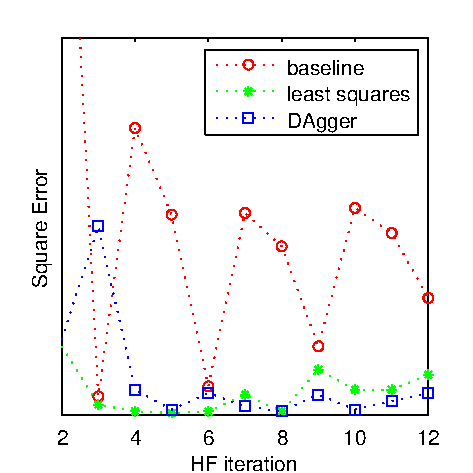
\includegraphics[scale=0.7]{propylsub_pzero_test_12iter.pdf}
  \caption{$\rho_0 = 0$}
  \label{fig:propSub0}
\end{subfigure}%
\begin{subfigure}{.5\textwidth}
  \centering
  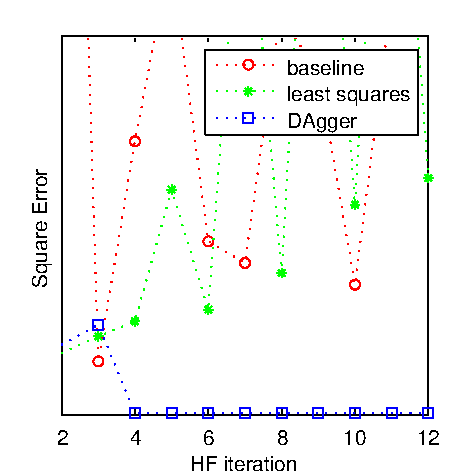
\includegraphics[scale=0.7]{propylsub_peye_test_12iter.pdf}
  \caption{$\rho_0 = I$}
  \label{fig:propSubI}
\end{subfigure}
\caption{Error as a function of iteration tested on \textit{pentPropylF} dataset}
\label{fig:testpropSub}
\end{figure}

Evaluating the robustness of these policies by testing on datasets consisting of a different class of molecules are shown in Figure~\ref{fig:testcycloPen} and \ref{fig:testpropSub}. Least squares does not perform as good as DAgger in these cases, this could be due to tendency to over-fit. DAgger provides also a more robust set of coefficients given that it is trained on two different initial guess density matrices ($\rho_0 = 0$ and $\rho_0 = I$).



\section{CONCLUSION}
In the experiment, we first proposed the least squares policy. It is easy to train and already can yield much lower error comparing to the baseline. However, it tend to somewhat over-fit the training data and performance fluctuates on testing data accordingly. On the other hand, DAgger does train a more robust policy which is more flexible with input initial guess. DAgger outperforms least squares when tested on different datasets.  
During the training process in DAgger, it keeps aggregating the dataset hence has a more diverse training instances. This can prevent the policy from over-fitting the training dataset thus produces a more stable and smooth decreasing trend. This provides a great property when dealing with large molecules or on the case which is hard to get to convergence.

\bibliography{refs}

\end{document}





%Figure \ref{fig:testZero} shows the error of each policy on the cycloPentene testing dataset for 12 iterations. The baseline is the policy that always uses the average of the last two density matrices to serve as the input to the next iteration.  
%
%We can observe that all the policies seems to converge within 10 iterations except the baseline fluctuates.


%The baseline again fluctuates while all the other policies still converges within 12 iteration. 
%Least squares and DAgger got pretty similar error after 12 iterations.
%
%However, the performance of linear combination fluctuates during iteration 5 - 10 while both DAgger with different experts have a more steady decreasing trend across all 12 iterations. 


%\begin{figure}[h!]
%\center
%  \caption{Absolute value of difference between iterations on training dataset}
%	\label{fig:converge_training}
%    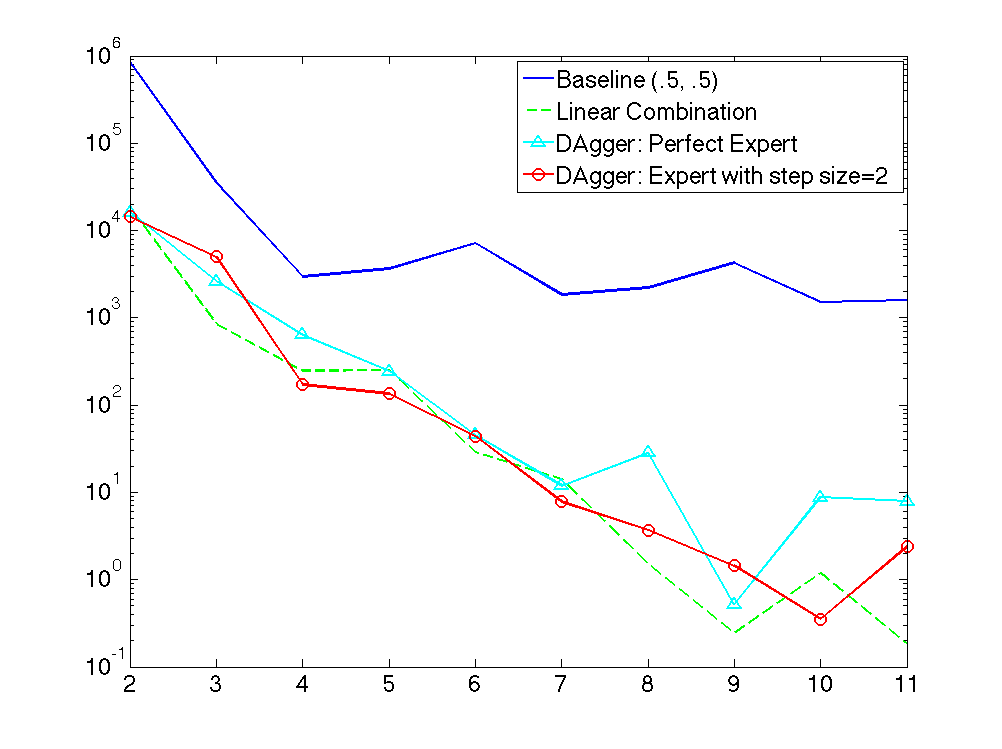
\includegraphics[width=210px]{convergence_Training.png}
%\end{figure}
%
%\begin{figure}[h!]
%\center
%  \caption{Absolute value of difference between iterations on testing dataset}
%  \label{fig:converge_testing}
%    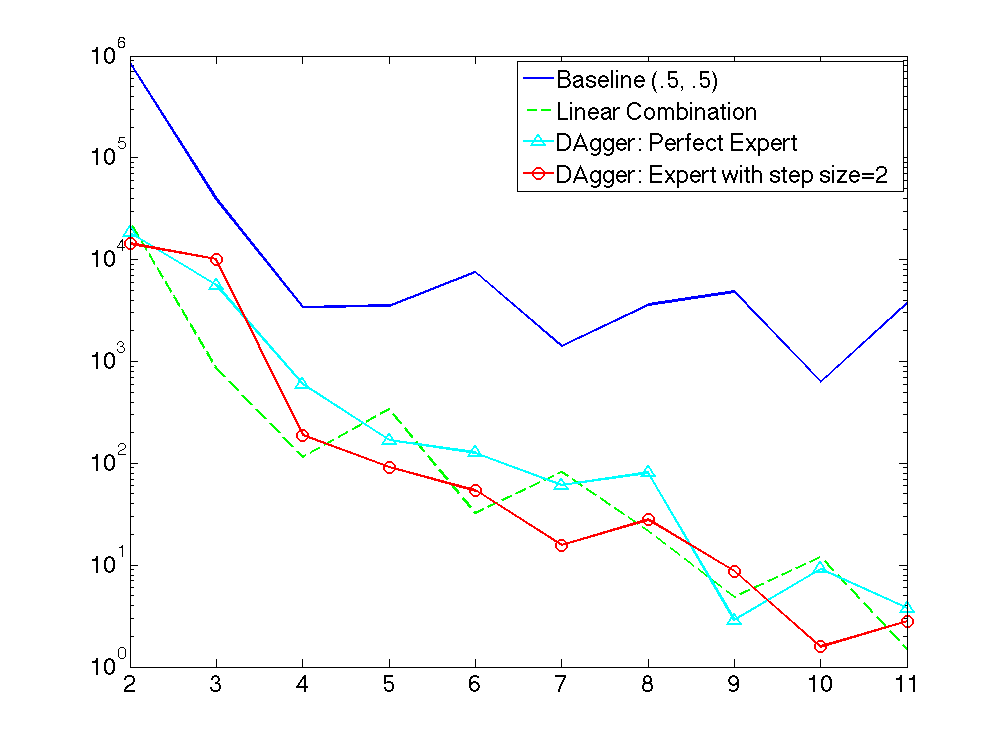
\includegraphics[width=210px]{convergence_Testing.png}
%\end{figure}


%Compare to the result on the training dataset (Figure \ref{fig:training}), the curves are similar for DAgger and baseline, but is pretty different for the least squares. Least squares performs the best and has a smooth result on training dataset while it fluctuates on testing dataset. It is possible because of the least squares over-fit the training dataset. On the contrary, DAgger with the expert that has step size of 2 got more consistent results between training and testing dataset.
%
%

%\begin{figure}[h!]
%\centering
%\begin{subfigure}{.5\textwidth}
%  \centering
%  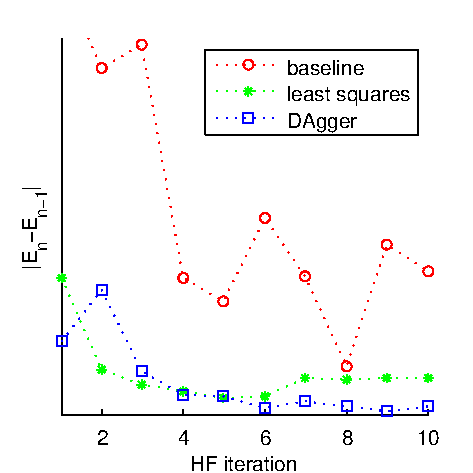
\includegraphics[scale=0.7]{dE_cycloPen_pzero_test_12iter.pdf}
%  \caption{$\rho_0 = 0$}
%  \label{fig:sub1}
%\end{subfigure}%
%\begin{subfigure}{.5\textwidth}
%  \centering
%  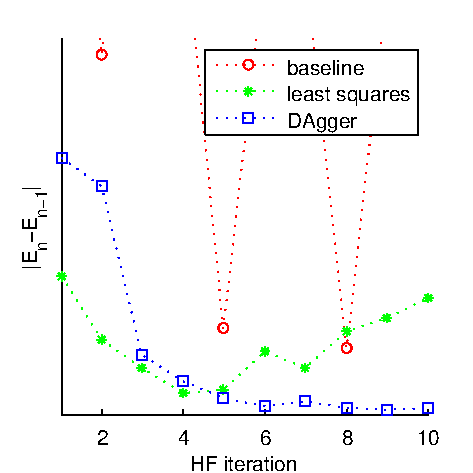
\includegraphics[scale=0.7]{dE_cycloPen_peye_test_12iter.pdf}
%  \caption{$\rho_0 = I$}
%  \label{fig:sub2}
%\end{subfigure}
%\caption{Error as a function of iteration for test on \textit{cycloPentene} dataset}
%\label{fig:test}
%\end{figure}